\begin{figure*}
    \begin{minipage}[t]{0.51\textwidth}
        \centering
        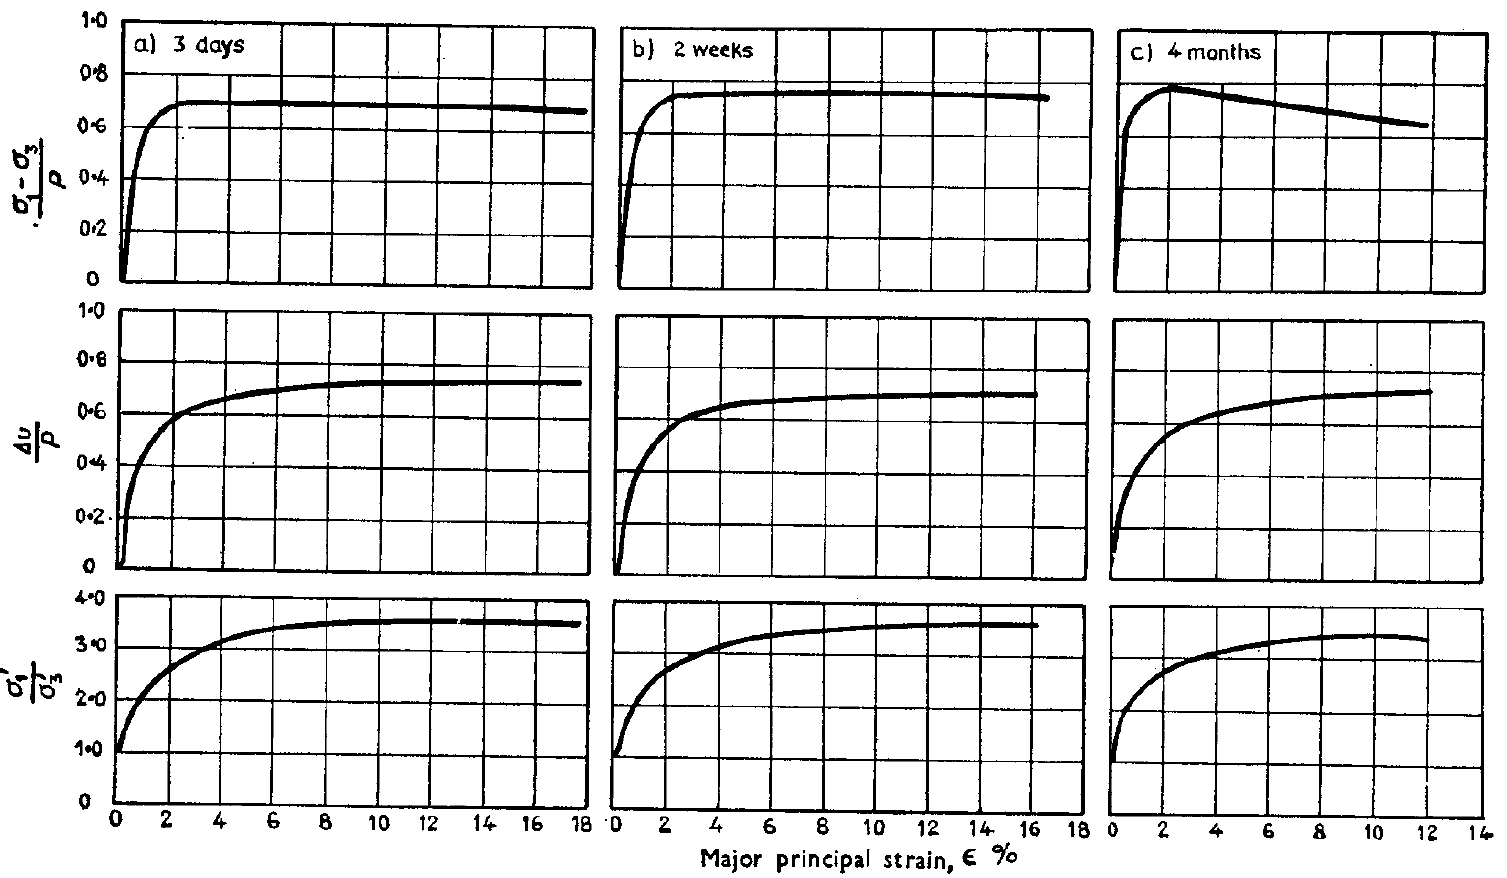
\includegraphics[width=\textwidth]{figures/figure-2.png}
        \caption{Results of consolidated undrained triaxial tests on samples consolidated isotropically for various periods of times: (a) 3 days, (b) 2 weeks, (c) 4 months. Consolidation pressure 25 $\rm{kg/sq\cdot{cm}}$. Each curve represents the average of two tests.}
        \addtocounter{figure}{-1}
        \vspace{-5pt}
        \renewcommand{\figurename}{图}
        \caption{各向同性固结样品在不同时间段的固结不排水三轴试验结果:(a)3天,(b)2周,(c)4个月。 固结压力25$\rm{kg/sq\cdot{cm}}$。 每条曲线代表两次试验的平均值。}
        \renewcommand{\figurename}{Figure}
        \label{figure:2}
    \end{minipage}
    \begin{minipage}[t]{0.44\textwidth}
        \centering
        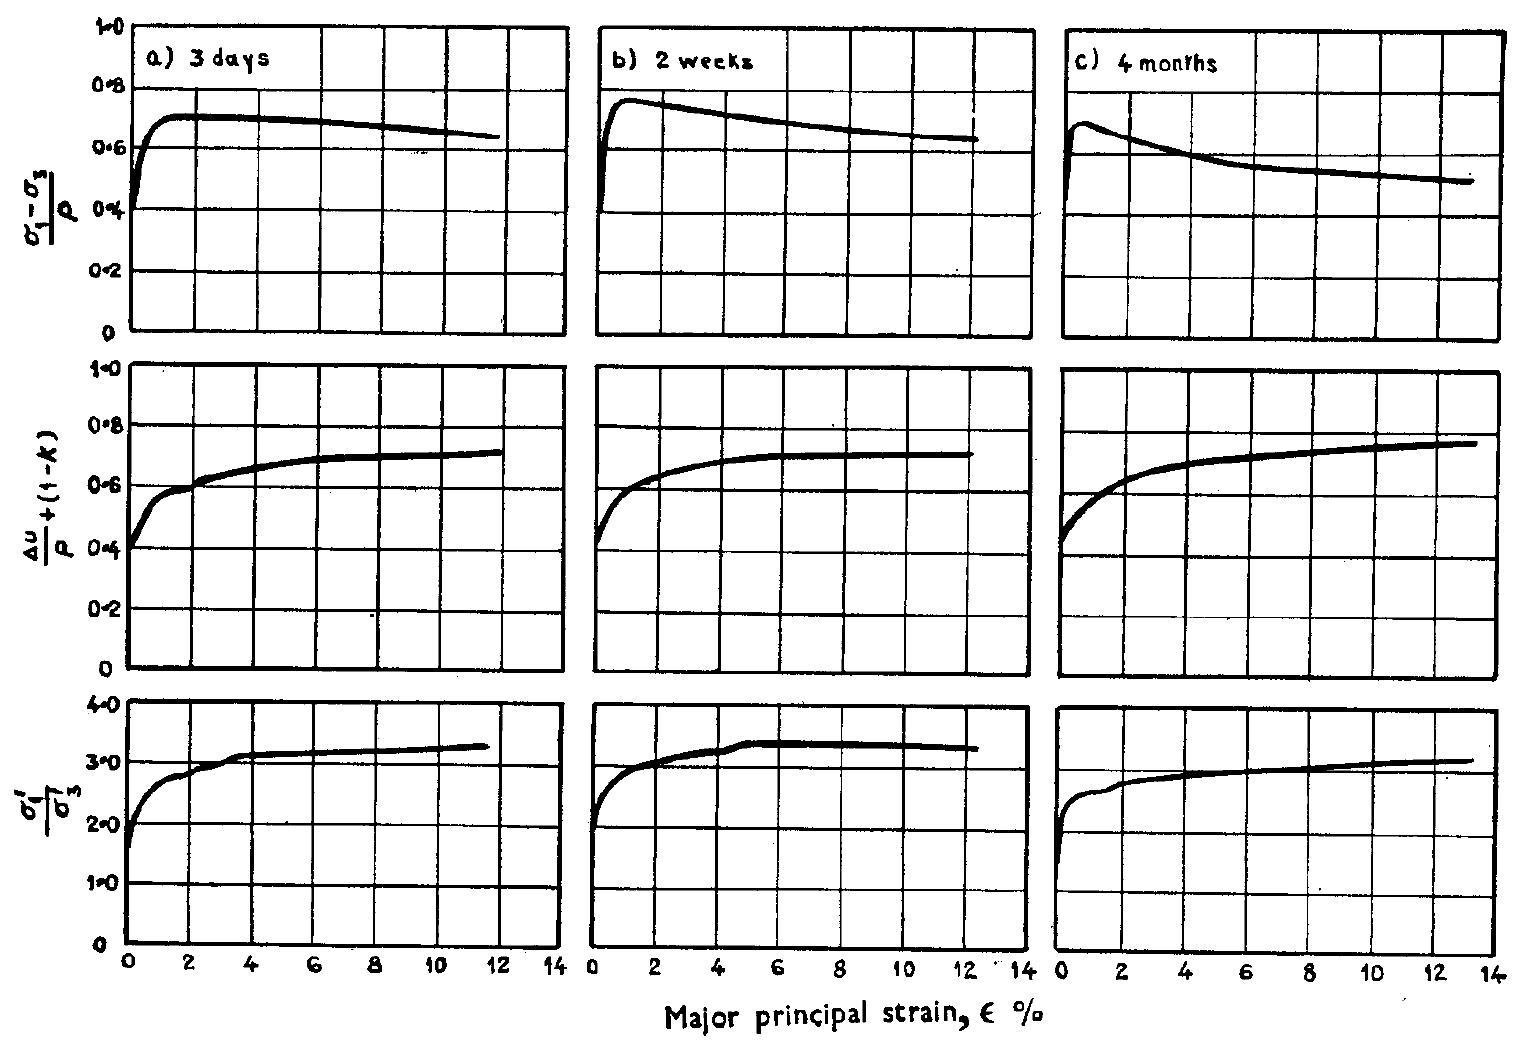
\includegraphics[width=\textwidth]{figures/figure-3.png}
        \caption{Results of consolidated undrained triaxial tests on samples consolidated anisotropically for various periods of times: (a) 3 days, (b) 2 weeks, (c) 4 months.
        Consolidation pressure $p_1=2.5\rm{kg/sq\cdot{cm}},p_2=p_3=1.5\rm{kg/sq\cdot{cm}}$. Each curve represents the average of two tests}
        \addtocounter{figure}{-1}
        \vspace{-5pt}
        \renewcommand{\figurename}{图}
        \caption{在不同时间段进行各向异性固结的样品的固结不排水三轴试验结果:(a)3天,(b)2周,(c)4个月。固结压力$p_1=2.5\rm{kg/sq\cdot{cm}},p_2=p_3=1.5\rm{kg/sq\cdot{cm}}$。每条曲线代表两次试验的平均值}
        \renewcommand{\figurename}{Figure}
        \label{figure:3}
    \end{minipage}
\end{figure*}